

%\documentclass[hyperref={pdfpagelabels=false}]{beamer}
\documentclass[11pt]{beamer}
\usepackage{beamerthemesplit}
\usepackage[T1]{fontenc}
\usepackage[utf8]{inputenc}
\usepackage{enumerate}
\usepackage{amsmath,amssymb,amsthm}
\usepackage{graphicx}
\usepackage{tikz}
\usepackage{eurosym}
\usepackage[round]{natbib}
\usepackage{subfigure}
\usepackage{array}
\usepackage{booktabs}
\usepackage{listings}
\usepackage{bbold}
\bibliographystyle{chicago}
%\def\bibfont{\scriptsize}
%\renewcommand{\bibsection}{\subsubsection*{\bibname } }
\renewcommand\bibsection{\section[]{\refname}}

\title[]{{\small Recherche des consommateurs et dispersion des prix: analyses du marché des carburants et de la grande distribution en France}}
\author[]{\small Etienne Chamayou}
\institute{Soutenance de Thèse - Université Paris Saclay, le 21 septembre 2017}
\date{}

\begin{document}
\frame{\titlepage
\small Jury:
{\scriptsize
\begin{itemize}
\item Francis Bloch, Université Paris 1-PSE (Directeur de Thèse)
\item Philippe Gagnepain, Université Paris 1-PSE (Rapporteur)
\item Erwan Gautier, Université de Nantes-Banque de France (Rapporteur)
\item Claire Chambolle, Inra-Ecole Polytechnique (Examinateur)
\item Thibaud Vergé, Crest-Ensae (Examinateur)
\end{itemize}
}
}

\section{Introduction}

\frame{\frametitle{De la loi du prix unique à la dispersion des prix}
Un cadre de référence: la concurrence pure et parfaite:
\begin{itemize}
	\item Homogénéité du produit
	\item Transparence de l'information
\end{itemize}
=> Loi du prix unique
\ \\
\ \\
Litérature sur la dispersion des prix et des coûts de recherche:
\begin{itemize}
\item \cite{STI61}: «One should hardly have to tell academicians that information is a valuable ressource (...) and yet it occupies a slum dwelling in the town of economics»
\item \cite{VAR80}: «Economists have belatedly come to recognize that the "law of one price" is no law at all»
\end{itemize}
=> Quid de l'efficience des marchés?
}

\frame{\frametitle{Dispersion des prix et coûts de recherche des consommateurs}
\cite{STI61}: «Price dispersion is a manifestation - and, indeed, it is the measure - of ignorance in the market»
\begin{itemize}
\item L'information des consommateurs est a priori difficile à caractériser
\item A contrario: la dispersion des prix est mesurable
\end{itemize}
L'observation des prix permet potentiellement de caractériser les comportements de recherche des consommateurs sur un marché
\ \\
\ \\
Enjeux en termes de politiques publiques:
\begin{itemize}
\item Favoriser la transparence des marchés
\item Contrôle des concentrations
\end{itemize}
}

\frame{\frametitle{Démarche de recherche}
Analyse de la concurrence en France:
\begin{itemize}
\item entre les stations service
\item dans la grande distribution
\end{itemize}
à l'aune de la litérature théorique qui étudie le lien entre dispersion des prix et information imparfaite des consommateurs
\ \\
\ \\
Contributions:
\begin{itemize}
\item Création de deux larges jeux de données de prix à partir de données collectées en ligne => publication des données
\item Validation et discussion des modèles théoriques existants
\item Etat des lieux de la concurrence sur les marchés analysés
\end{itemize}
}

\section{La concurrence entre les stations services}

\frame{\frametitle{Data}
Source et préparation:
\begin{itemize}
\item Lancement en 2006 d'un site de comparaison des prix du carburant à l'initiative du Ministère de l'Economie, avec obligation légale de renseigner les prix pour les stations service dépassant un certain volume de ventes
\item Utilisation d'un script pour collecter les prix et les enseignes de manière quotidienne entre Septembre 2011 et Décembre 2014
\item Réconciliation des séries de prix, fiabilisation de l'information sur la localisation des stations
\item Base de données décrivant les prix de près de 10,000 stations services en France sur 3 ans
\end{itemize}
Axes de recherche:
\begin{itemize}
\item Etude d'un choc: création d'une enseigne à bas coût
\item Etude de la dispersion des prix "à l'équilibre"
\end{itemize}
}

\frame{\frametitle{Chapitre 1: Impact de la réation d'une enseigne à bas coût}
On distingue principalement deux types d'enseignes sur le marché français du carburant:
\begin{itemize}
\item Compagnies pétrolières: en retrait
\item Supermarchés: légère croissance
\end{itemize}
\ \\
\ \\
Création en 2011 par le groupe Total d'une chaine de stations services à bas prix, Total Access, à partir de:
\begin{itemize}
\item 280 stations Elf (prix bas avant conversion)
\item 300 stations Total (baisse de prix significative)
\end{itemize}
=> Sélection de stations aptes à compenser la baisse de marge par une hausse des volumes
}

\frame{\frametitle{Chapitre 1: Le réseau Total Access fin 2014}
\begin{figure}[h]
	\centering
		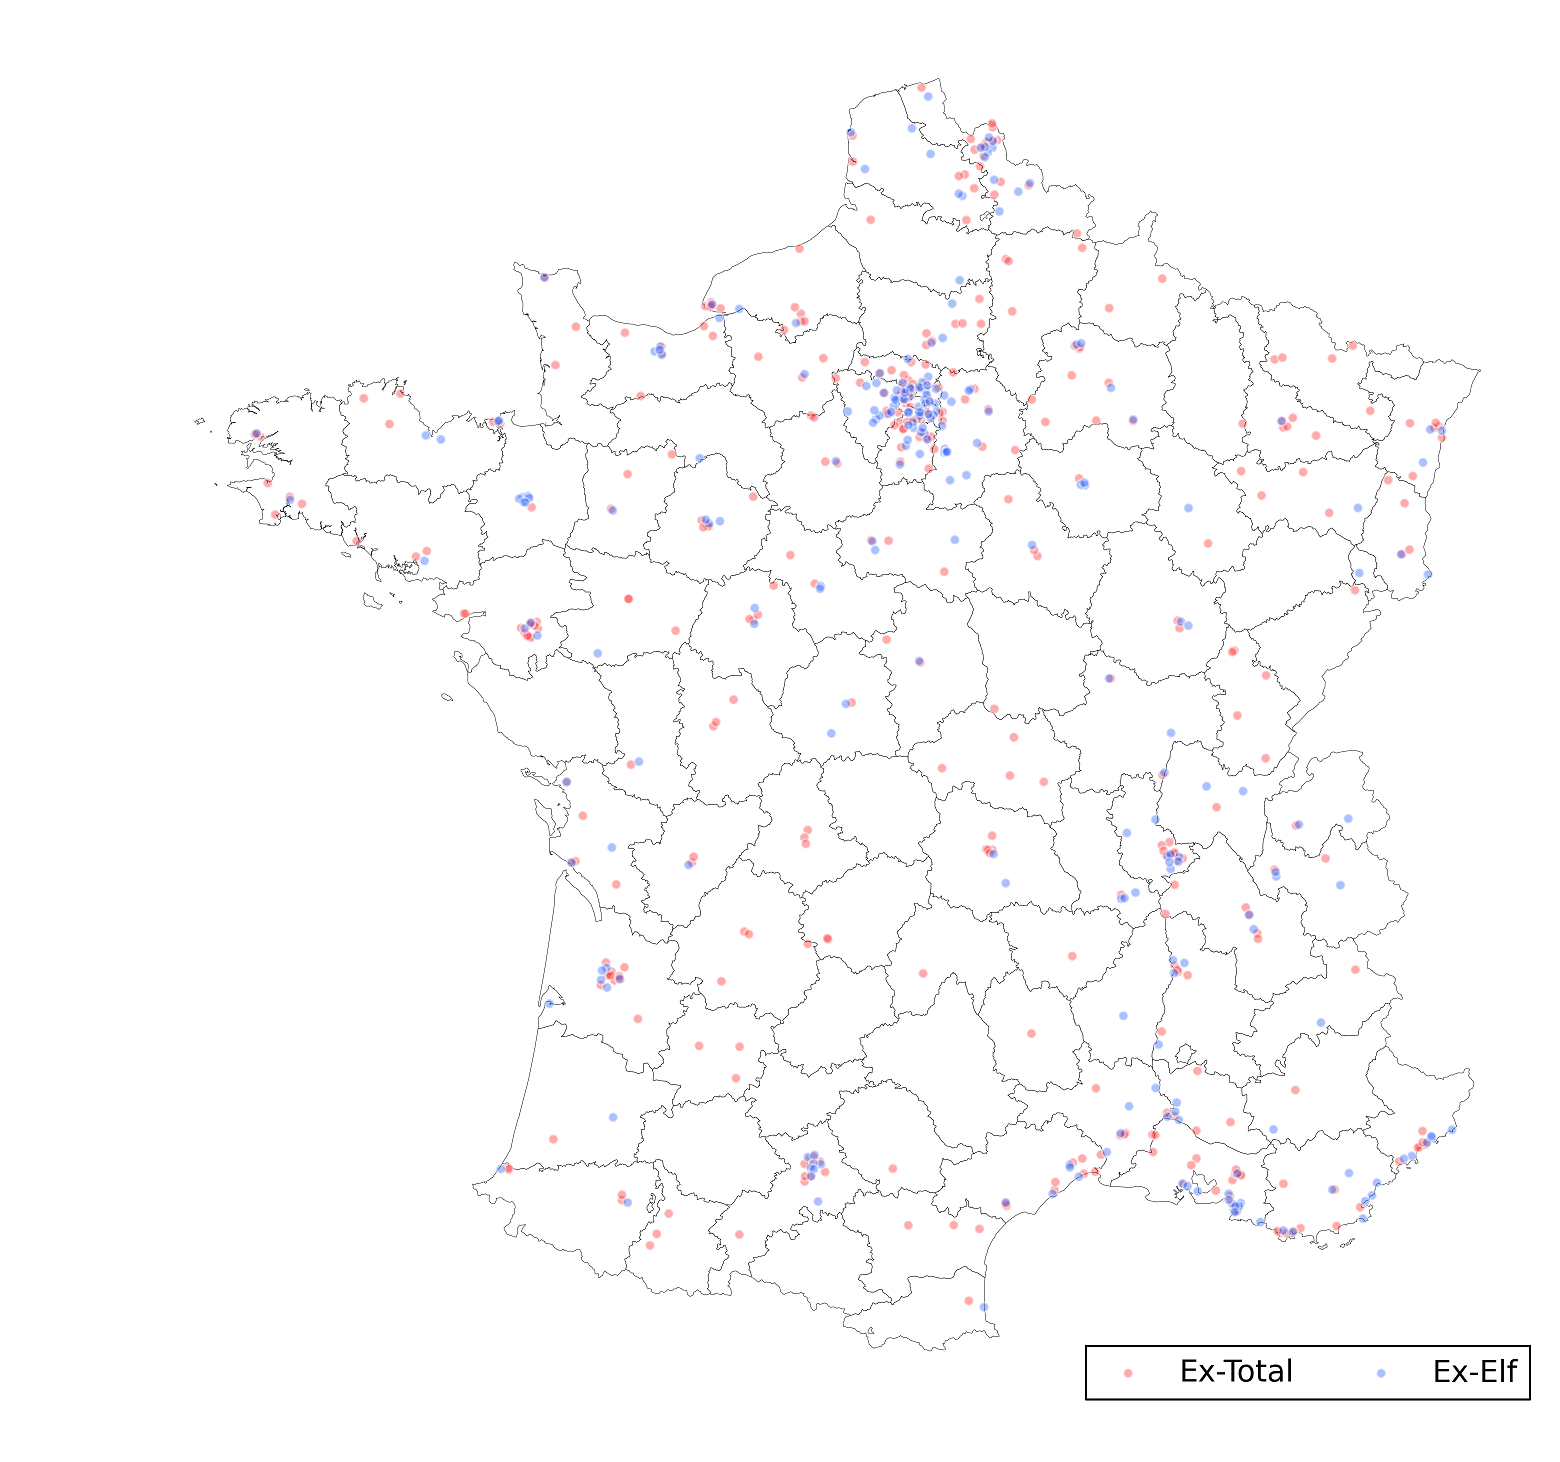
\includegraphics[width=7cm]{sketches/map_total_access_lq.png}
	\label{fig:price_vs_cost}
\end{figure}
}

\frame{\frametitle{Chapitre 1: Changement d'enseigne et de prix}
\begin{figure}[h]
	\centering
		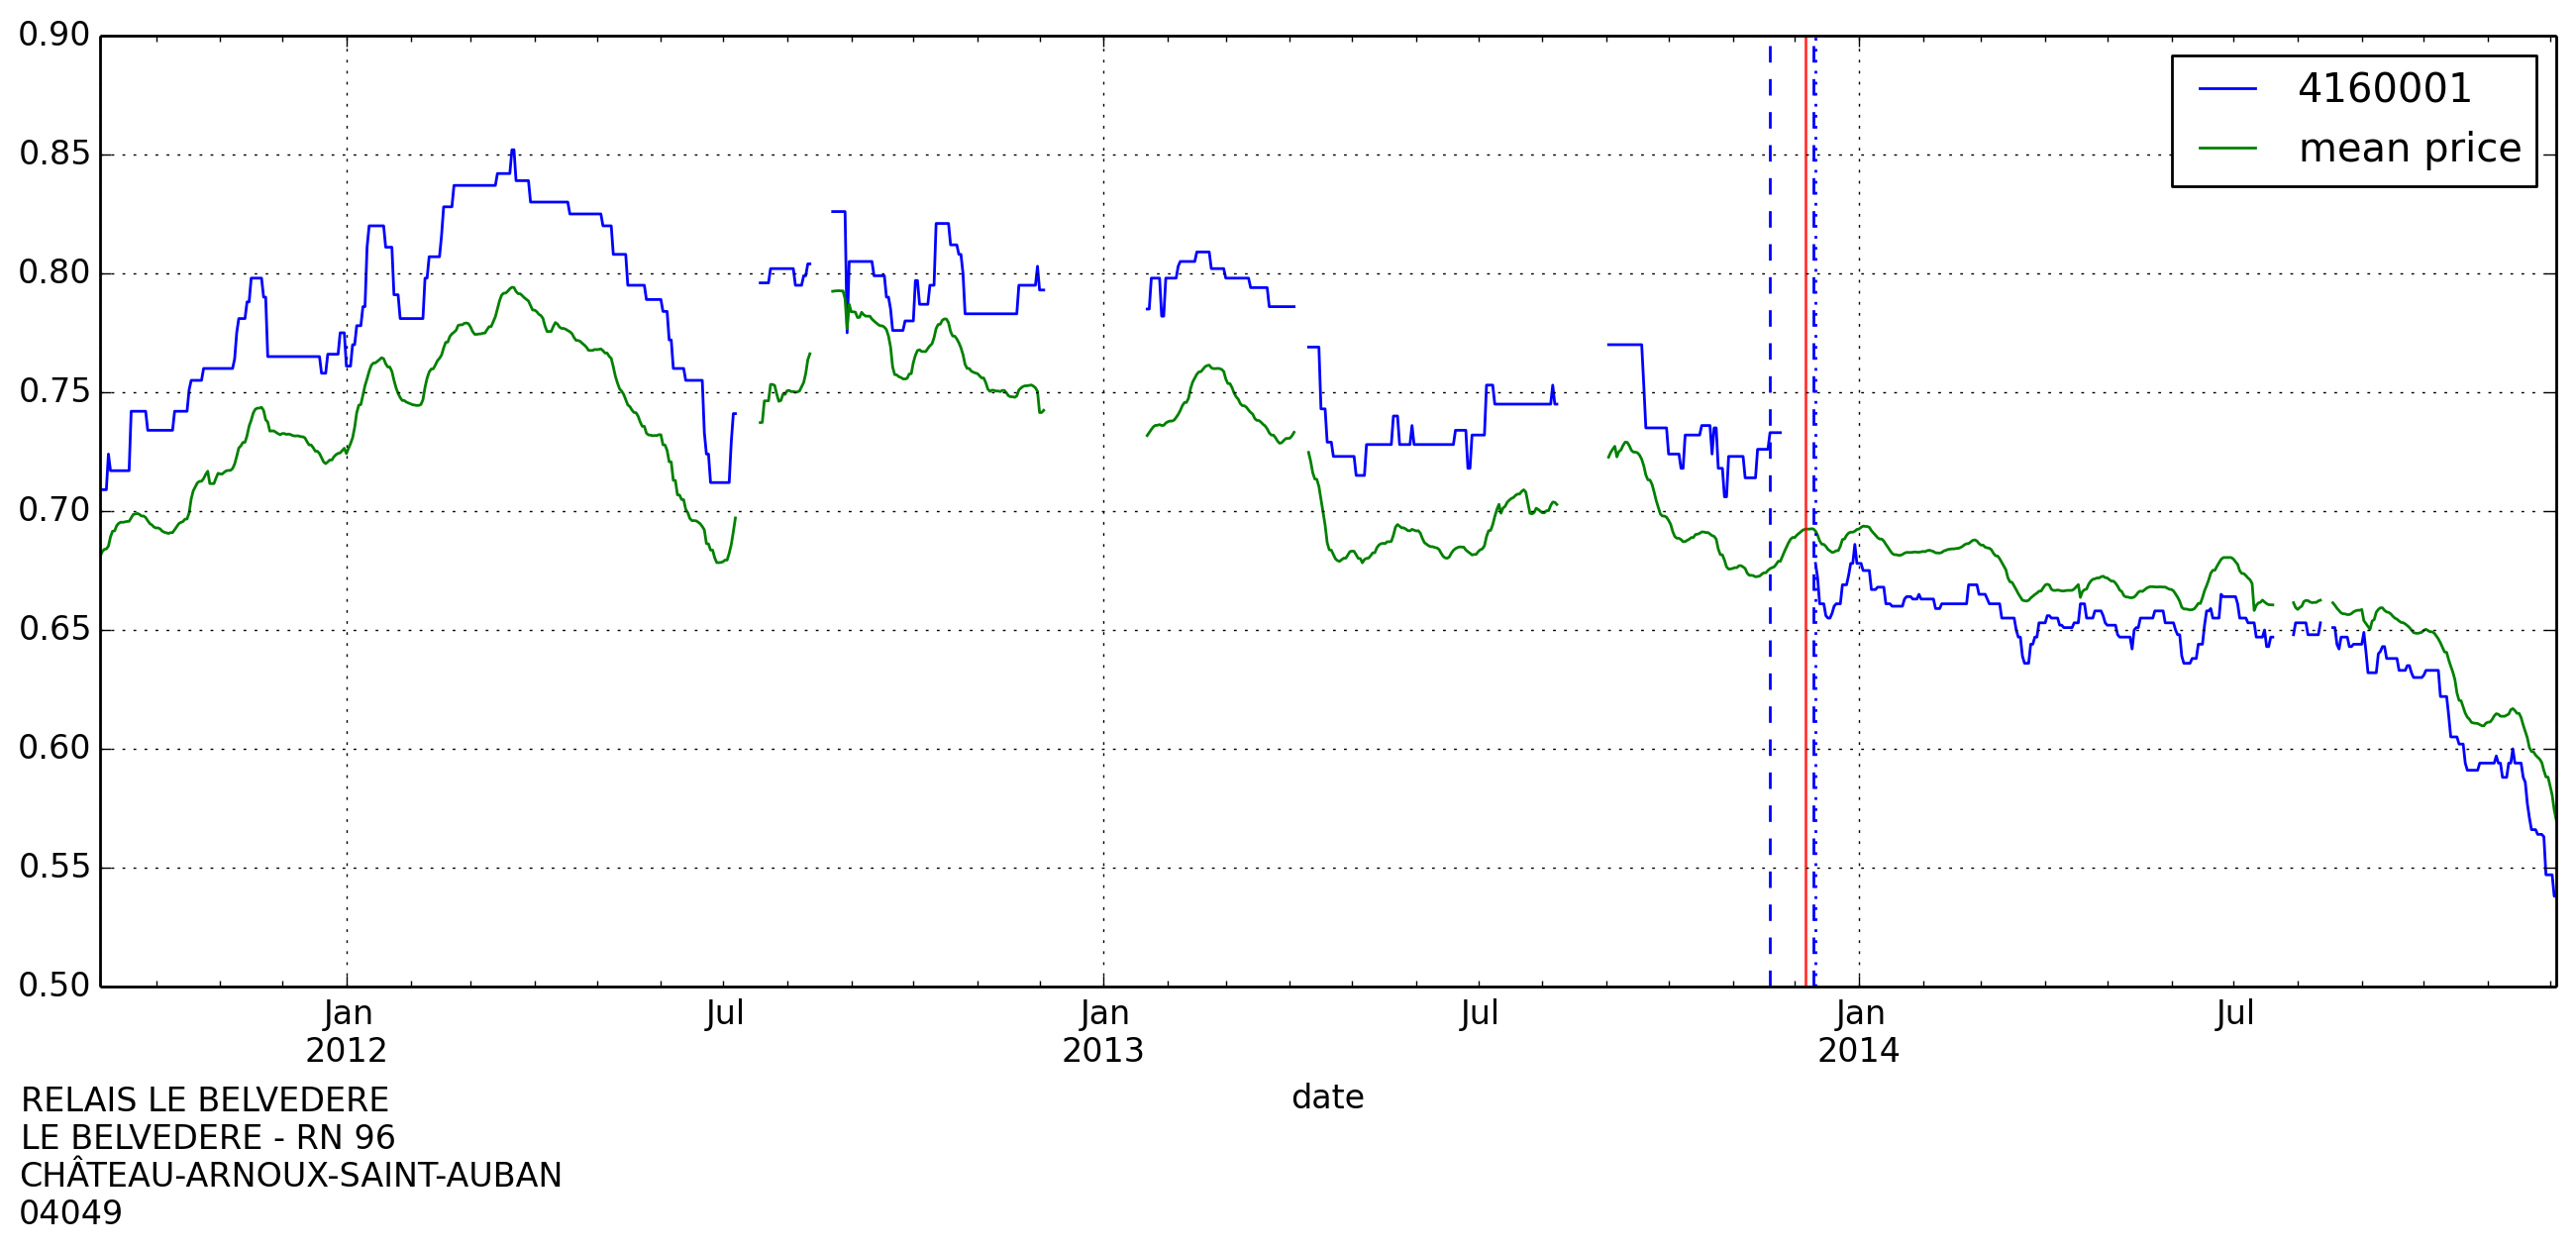
\includegraphics[width=11.5cm]{sketches/TOTAL_4160001_0062.png}
	\label{fig:price_vs_cost}
\end{figure}
}

\frame{\frametitle{Chapitre 1: Méthode}
Analyse de la réaction des proches concurrents à l'aide de la méthode des doubles différences:
\begin{itemize}
\item De manière agrégée au niveau national
	\begin{itemize}
	\item Concurrent si à proximité d'une station convertie
	\item Contrôle si dans le voisinage mais pas trop proche d'une station convertie
	\end{itemize}
\item En considérant chaque station individuellement
  \begin{itemize}
	\item Groupe de contrôle différent pour chaque station
	\item Investigation dans un deuxième temps des facteurs potentiellement explicatifs de l'hétérogénéité des réactions
\end{itemize}
\end{itemize}
}

\frame{\frametitle{Chapitre 1: Résultats et discussion}
\begin{itemize}
\item Faible réaction agrégée, inférieure à 1 centime d'euro par litre
\item Masque de l'hétérogénéité: parmi les 40\% de stations qui opèrent un ajustement:
\begin{itemize}
\item Baisses principalement implémentées par des stations d'enseignes de grande distribution => Marché fortement concurrentiel au préalable
\item Hausses chez des indépendants ou enseignes de groupes pétroliers => Contraintes de capacités et/ou localisation qui conduisent à se focaliser sur des consommateurs captifs
\end{itemize}
\item Prolongements: fermetures de stations supplémentaires? impact pour le consommateur?
\end{itemize}
}

\frame{\frametitle{Chapitre 2: Dispersion des prix et recherche des consommateurs}
\begin{itemize}
\item \cite{VAR80}: la présence de consommateurs parfaitements informés et de consommateurs faisant face à des coûts de recherche implique une absence d'équilibre en stratégies pures
\begin{itemize}
\item les vendeurs tirent leur prix dans une distribution à l'équilibre ce qui génère de la dispersion des prix
\item la dispersion est décroissante du coût marginal 
\item la dispersion est croissante du nombre de vendeurs
\end{itemize}
\item Empiriquement, on examine:
\begin{itemize}
\item La présence de changements de rang dans les prix des stations
\item La relation entre changements de rang et information des consommateurs
\item L'impact des fluctuations du coût de la matière première
\item L'hétérogénéité des situations de concurrence à l'échelle locale
\end{itemize}
\end{itemize}
}

\frame{\frametitle{Chapitre 2: Localisation des stations service de Marvejols}
\begin{figure}[h]
	\centering
		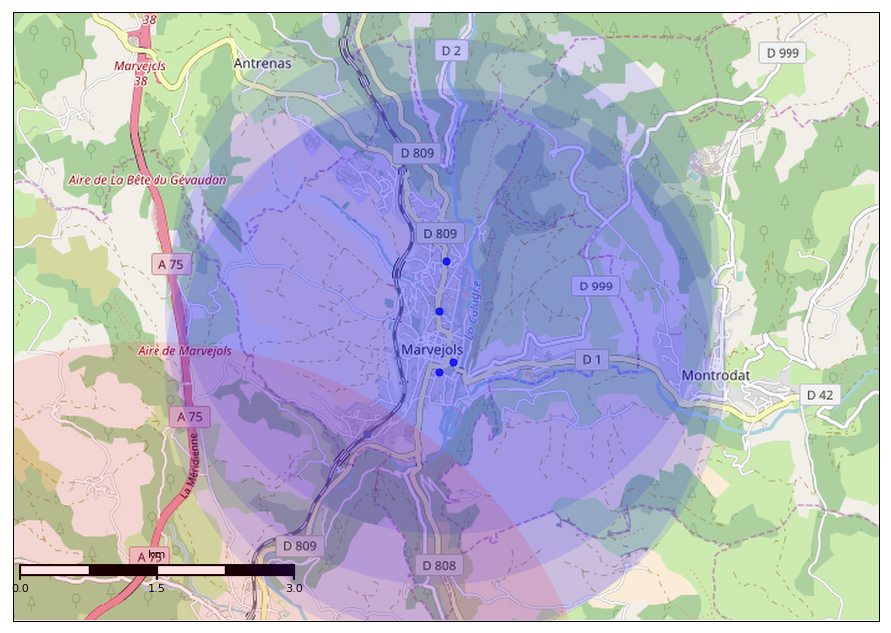
\includegraphics[width=7cm]{sketches/case_study_marvejols_map.png}
	\label{fig:price_vs_cost}
\end{figure}
}

\frame{\frametitle{Chapitre 2: Prix des stations services de Marvejols}
\begin{figure}[h]
	\centering
		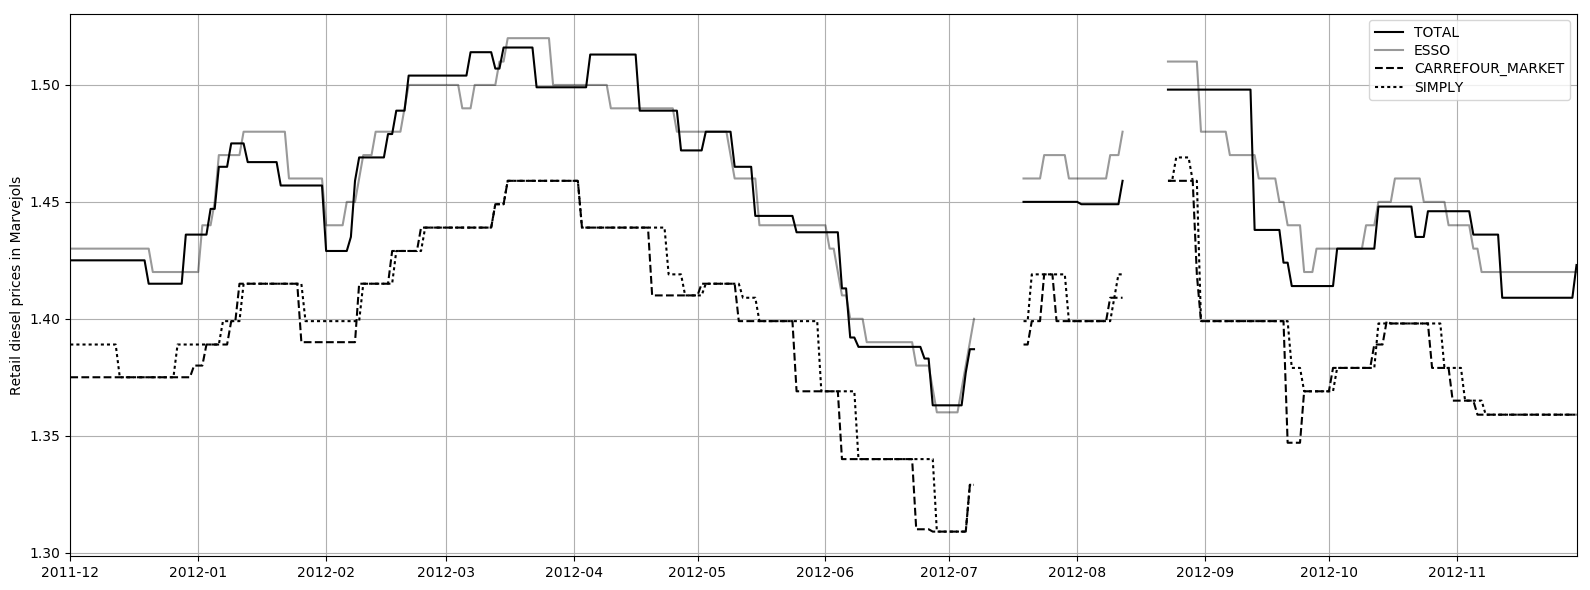
\includegraphics[width=11.5cm]{sketches/case_study_marvejols_prices.png}
	\label{fig:price_vs_cost}
\end{figure}
}

\frame{\frametitle{Chapitre 2: Méthode}
\begin{itemize}
\item Construction de statistiques décrivant la dispersion des prix entre les paires de stations concurrentes. Celles-ci motivent deux approches:
\begin{itemize}
\item Changements de rang (pétroliers et indépendants): Test proposé par \cite{TAP11}: régression de la dispersion sur une variable indicatrice qui distingue les paires de stations suffisamment proches pour que les frictions informationnelles deviennent négligeables
\item Alignement des prix (grande distribution): Test binomial d'égalité des probabilités d'adopter le même prix que le concurrent puis catégorisation des stations en agrégeant les résultats à travers les paires dont elles font partie
\end{itemize}
\item Régression d'indicateurs de dispersion mesurés quotidiennement et localement sur le coût de la matière première et le nombre de concurrents
\end{itemize}
}

\frame{\frametitle{Chapitre 2: Résultats et discussion}
Pétroliers et indépendants: résultats cohérents avec \cite{VAR80}
\begin{itemize}
\item Présence de changements de rang
\item Changements de rang moins fréquents parmi les stations très proches l'une de l'autre
\item Au niveau des marchés locaux, la dispersion des prix est:
\begin{itemize}
\item Négativement corrélée avec le coût d'approvisionnement
\item Positivement corrélée avec le nombre de stations
\end{itemize}
\end{itemize}
\ \\
\ \\
Grande distribution: concurrence à la Bertrand?
\begin{itemize}
\item Fort alignement des prix
\item Corrélation forte entre l'enseigne et la tendance à adopter le prix d'un concurrent ou d'être imité
\item Au niveau du marché: pas d'impact significatif du nombre de concurrents et des flucuations de coûts d'approvisionnements 
\end{itemize}
}

\section{La grande distribution}

\frame{\frametitle{Chapitre 3: Introduction}
\begin{itemize}
\item Concurrence entre supermarchés: chaque consommateur achète généralement une multitude de produits
\begin{itemize}
\item Comparaison des prix plus complexe
\item Différences d'assortiment, promotions, programmes de fidélités
\end{itemize}
\item Peu de modèles théoriques sur la dispersion des prix dans le cas multi-produits (\cite{MCA95}: Equilibres en stratégies mixtes)
\item Peu de données disponibles, encore moins dans le domaine public (\cite{BIS13}, \cite{PER15}, \cite{ALL16b})
\end{itemize}
}

\frame{\frametitle{Chapitre 3: Data}
Source et préparation:
\begin{itemize}
\item Création du comparateur de prix quiestlemoinscher.com par Leclerc en 2006
\begin{itemize}
	\item Comparaisons agrégées entre enseignes jusqu'en 2012
	\item Comparaisons de magasins concurrents à partir de 2013
\end{itemize}
\item Utilisation d'un script pour collecter tous les prix disponibles sur le site en Mars 2015: cross section de 4 millions de prix couvrant 2,300 supermarchés
\item Récupération de données de prix datant de Mai 2014 (pdf)
\item Données LSA: variables de concurrence
\end{itemize}
Axes de recherche:
\begin{itemize}
\item Explication des prix par les caractéristiques des magasins et marchés locaux
\item Etude de la dispersion des prix
\end{itemize}
}

\frame{\frametitle{Chapitre 1: Comparaisons nationales}
\begin{figure}[h]
	\centering
		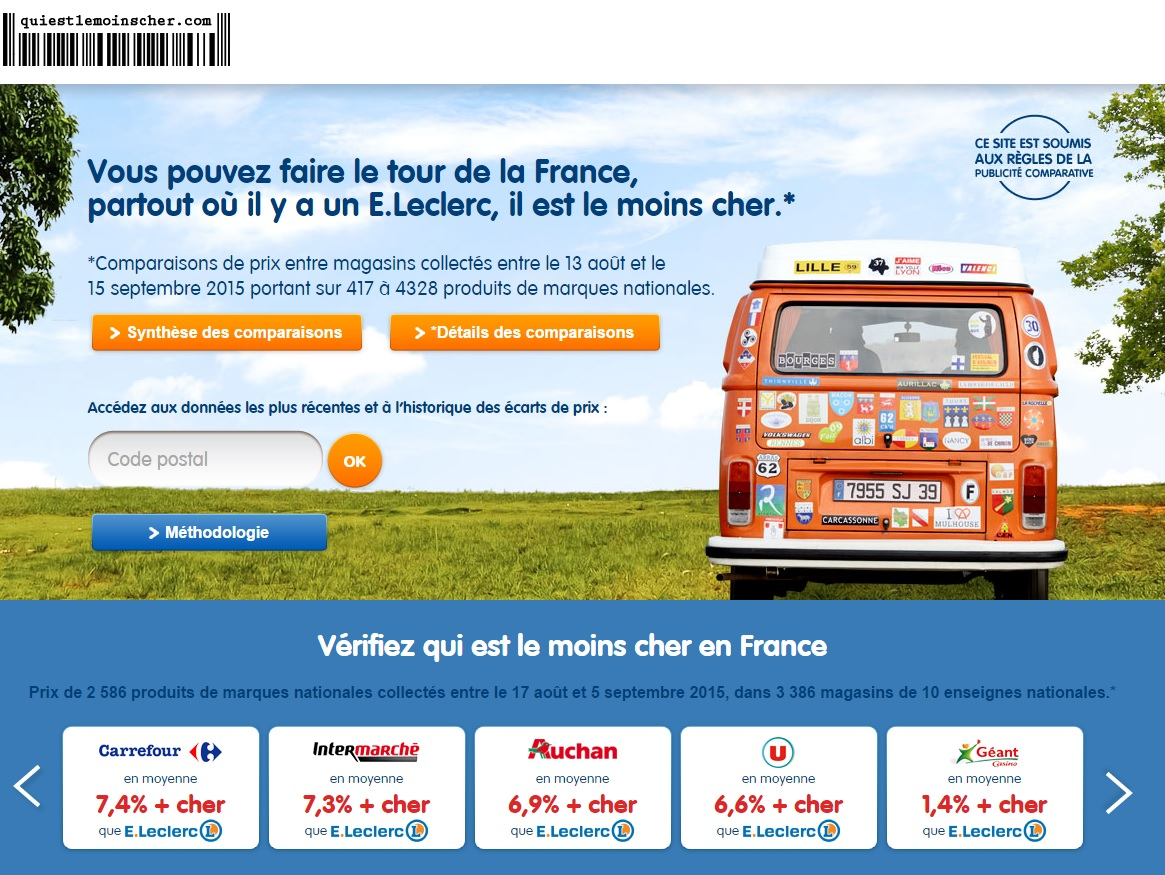
\includegraphics[width=7cm]{sketches/qlmc_national.jpg}
	\label{fig:qlmc_national}
\end{figure}
}

\frame{\frametitle{Chapitre 1: Comparaisons locales}
\begin{figure}[h]
	\centering
		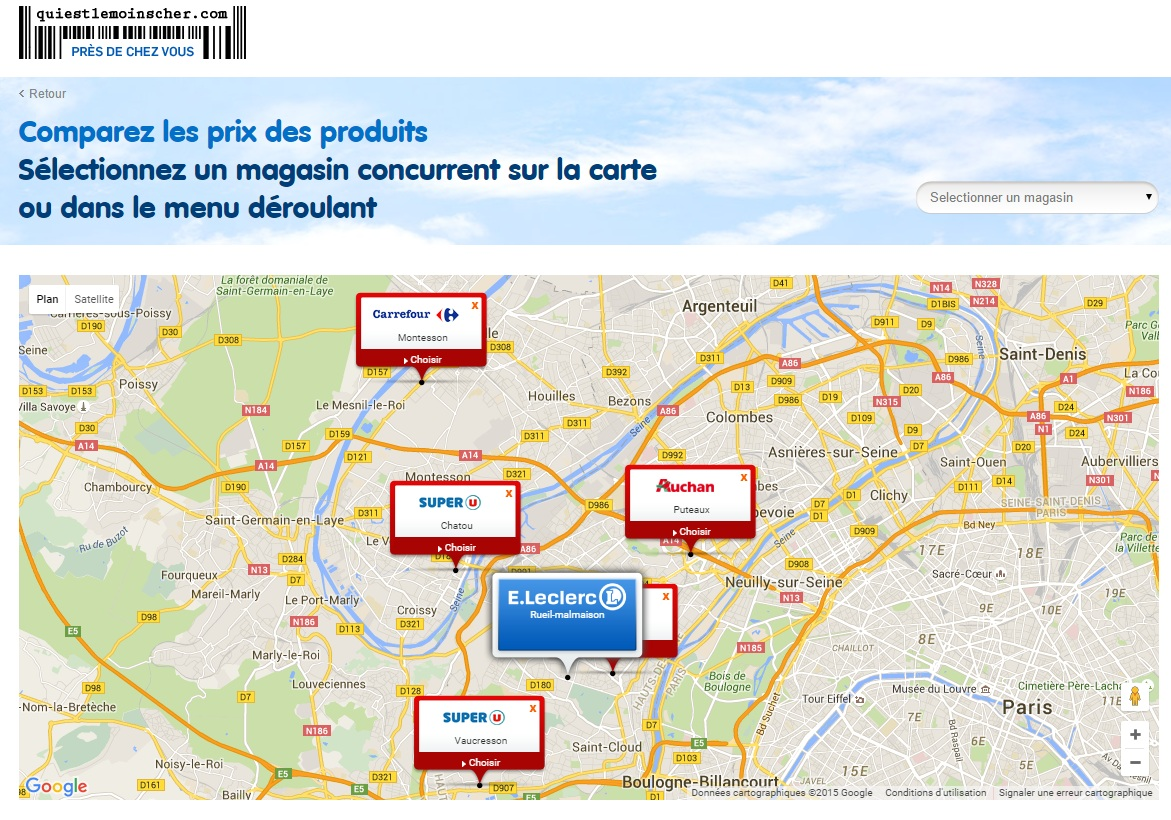
\includegraphics[width=7cm]{sketches/qlmc_competitor_selection.jpg}
	\label{fig:qlmc_competitor_selection.jpg}
\end{figure}
}

\frame{\frametitle{Chapitre 3: Méthode}
\begin{itemize}
\item Etude des déterminants des prix
\begin{itemize}
\item Construction d'un index prix par magasin
\item Approximation du HHI par la surface, avec ou sans pondération par la distance (chaque magasin est considéré comme le centre d'un marché)
\item Analyse de l'hétérogénéité des prix intra-enseigne
\end{itemize}
\item Etude de la dispersion
\begin{itemize}
\item Calcul de statistiques de changements de rangs statiques et dynamiques entre paires de magasins concurrents: test distance vs. changements de rang
\item Mesure de la dispersion à travers les marchés locaux: relation avec le niveau des prix
\end{itemize}
\end{itemize}
}

\frame{\frametitle{Chapitre 3: Résultats et discussion}
\begin{itemize}
\item Pas d'impact significatif du HHI (approximé) sur les prix
\item L'enseigne apparaît déterminante
\item Les enseignes dont les prix sont les plus bas sont les enseignes dont les prix sont les plus homogènes (proche du prix unique pour Géant Casino)
\item Les changements de rang statiques et dynamiques sont très fréquents
\item On retrouve un lien entre ces changements de rang et la distance comme dans le cas du carburant
\item Au niveau des marchés locaux, une plus forte dispersion est associée à des prix plus élevés
\end{itemize}
}

\section{Conclusion}

\frame{\frametitle{Conclusion}
\begin{itemize}
\item Ce travail s'appuie sur des données de prix fournies à la demande du régulateur mais également à l'initative d'une chaine de grande distribution pour analyser la concurrence entre les stations services ainsi qu'entre les supermarchés
\item Les résultats suggèrent que les coûts d'acquisition de l'information affectent les mécanismes de concurrence de manière significative
\item Ils encouragent à engager de nouvelles initiatives en faveur de la transparence des marchés... ainsi qu'un suivi de leurs effets!
\end{itemize}
}

\frame{\frametitle{Conclusion}
Merci de votre attention!
}

\appendix

\frame[allowframebreaks]{\frametitle{References}
\nocite{*}
\bibliography{references}
}

\end{document} 